%---------------------------------------------------------------------------%
%-                                                                         -%
%-                           LaTeX Template                                -%
%-                                                                         -%
%---------------------------------------------------------------------------%
%- Copyright (C) Huangrui Mo <huangrui.mo@gmail.com> 
%- This is free software: you can redistribute it and/or modify it
%- under the terms of the GNU General Public License as published by
%- the Free Software Foundation, either version 3 of the License, or
%- (at your option) any later version.
%---------------------------------------------------------------------------%
%->> Document class declaration
%---------------------------------------------------------------------------%
\documentclass{Style/ucasproposal}%
%- Multiple optional arguments:
%- [<oneside|twoside|print>]% oneside eprint, twoside eprint, or paper print
%- [fontset=<adobe|none|...>]% specify font set instead of automatic detection
%- [scheme=plain]% thesis writing of international students
%- [draftversion]% show draft version information
%- [standard options for ctex article class: draft|paper size|font size|...]%
%---------------------------------------------------------------------------%
%->> Document settings
%---------------------------------------------------------------------------%
\usepackage[authoryear,list,xhf]{Style/artratex}% document settings
%- usage: \usepackage[option1,option2,...,optionN]{artratex}
%- Multiple optional arguments:
%- [bibtex|biber]% set bibliography processor and package
%- [<numbers|super|authoryear|alpha>]% set citation and reference style
%- <numbers>: textual: Jones [1]; parenthetical: [1]
%- <super>: textual: Jones superscript [1]; parenthetical: superscript [1]
%- <authoryear>: textual: Jones (1995); parenthetical: (Jones, 1995)
%- <alpha>: textual: not available; parenthetical: [Jon95]
%- [geometry]% reconfigure page layout via geometry package
%- [lscape]% provide landscape layout environment
%- [xhf]% disable header and footer via fancyhdr package
%- [color]% provide color support via xcolor package
%- [background]% enable page background
%- [tikz]% provide complex diagrams via tikz package
%- [table]% provide complex tables via ctable package
%- [list]% provide enhanced list environments for algorithm and coding
%- [math]% enable some extra math packages
%- [xlink]% disable link colors
\usepackage{Style/artracom}% user defined commands
%---------------------------------------------------------------------------%
%->> Document inclusion
%---------------------------------------------------------------------------%
%\includeonly{Tex/Chap_1,...,Tex/Chap_N}% selected files compilation
%---------------------------------------------------------------------------%
%->> Document content
%---------------------------------------------------------------------------%
%-
%-> Titlepage information
%-
\usepackage{makecell}
\counterwithin{figure}{section}
\counterwithin{table}{section}

%---------------------------------------------------------------------------%
%->> Titlepage information
%---------------------------------------------------------------------------%
%-
%-> 中文封面信息
%-
\schoollogo{scale=0.112}{ucas_logo}% 校徽
\title{面向微服务负载均衡的智能网关设计与实现}% 题目
\author{侯胜明}% 作者姓名
\authorid{2021E8015082032}% 学号
\advisor{陈伟}% 指导老师
\advisortitle{副研究员}% 指导老师职务
\degree{工学硕士}% 学位:硕士、博士
\degreetype{}% 学位类别:理学、工学、工程、医学等
\major{软件工程}% 二级学科专业名称
\field{分布式软件理论与技术}% 研究方向
\institute{中国科学院软件研究所}% 院所
\chinesedate{2023~年~06~月~16~日}
%\institute{中国科学院力学研究所\\流固耦合实验室}% 多行院所名称示例
%\chinesedate{2014~年~06~月~19~日}% 日期
%---------------------------------------------------------------------------%
%
\begin{document}
%-
%-> Frontmatter: title page, abstract, content list, symbol list, preface
%-
\pagenumbering{roman}% page numbers with roman style
%---------------------------------------------------------------------------%
%-> Frontmatter
%---------------------------------------------------------------------------%
%-
%-> 生成封面
%-
\maketitle% 生成中文封面

\section*{填表说明}
~\\
~\\
\begin{itemize}[leftmargin=*]
\item[1.] 本表内容须真实、完整、准确。
\item[2.] “学位类别” 名称填写:哲学博士、教育学博士、理学博士、工学博士、农学博士、医学博士、管理学博士, 哲学硕士、经济学硕士、法学硕士、教育学硕士、文学硕士、理学硕士、工学硕士、农学硕士、医学硕士、管理学硕士等。
\item[3.] “学科专业” 名称填写: “二级学科”全称。
\end{itemize}
\newpage
\section*{摘要}
为了实现服务灵活扩展,服务资源细化,服务快速升级等目的,软件体系结构转向了微服务结构,告别了传统的单体架构模式。微服务架构将整体服务拆分为一组小服务,小服务之间通过轻量级协议进行通信。随着微服务体量的增大,服务编排问题日益凸显,为了解决这个问题提出了服务网格的概念,意在使微服务系统获得伸缩能力与局部故障处理能力,由于技术的异构性,服务之间存在非常复杂的调用关系,怎么解决服务之间的调度是一个亟待解决的问题。针对这一问题,我们提出了一种在服务网格下对服务进行智能调度的方法,来提供更加完善的微服务调度方式提高微服务系统的整体响应能力。本方法分为三个部分,第一部分是基于多维度指标综合的动态负载计算,从多个维度去对服务实例负载进行计算和分析服务实例真正状态;第二部分是考虑细粒度版本兼容性的路由策略,通过更加细粒度的路由策略,将服务流量分流到更加合适的实例中;第三部分是两阶段的服务请求路由机制,通过两种不同着重点的网关之间的相互配合来实现更加灵活的服务请求路由方式。
\newpage
%-
%-> 目录
%-
\tableofcontents% 生成目录
%---------------------------------------------------------------------------%
% title page, abstract
%-
%-> Mainmatter
%-
\clearpage
\pagenumbering{arabic}% restart page numbers with arabic style
%---------------------------------------------------------------------------%
%->> Main content
%---------------------------------------------------------------------------%
\section{选题的背景及意义}

\subsection{选题背景}

随着微服务架构的高速发展,微服务架构成为当今分布式系统构建时的主流选择。微服务的发展经过了数代更替,在每个发展阶段中,微服务面临的挑战并不相同。云原生普及之前,微服务开发者专注的是微服务的架构、迭代、交付和运维。随着云原生技术的成熟,微服务也在被云原生化,这时候,开发者和架构师更关心的是如何借助云的优势,简化微服务的运维问题,并更专注在业务的交付效率上。

相比于传统的单体架构,微服务架构中服务异构性问题比较突出。为了快速的合作开发,微服务架构允许开发人员使用不同的语言框架构建单体小服务,服务之间通过REST API进行通信,此时外部客户端对于服务的请求就需要经过网关统一访问微服务集群,将服务请求处理,鉴权等工作由每个微服务集中到服务网关中进行实现。同时由于微服务规模的日益庞大,微服务的管理成为突出的问题,以此出现了服务编排,通过参数配置等简单的方式对微服务集群进行服务管理,例如Kubernetes等工具。在服务编排的基础上提出了服务网格,服务网格实现了请求在服务拓扑中的可靠穿梭,同时对应用是透明的,例如Istio等工具。

\subsubsection{REST API}

REST 由 Roy Fielding最早提出,是一种基于 HTTP 协议的软件架构风格。HTTP协议定义了 9 种标准方法,规定了客户端与服务器之间的信息交互方式。Fielding 发现对资源的四种常用操作方法(增删改查,CRUD)可以直接映射为 HTTP 协议的标准方法。由于与 HTTP 协议特性相吻合,REST 风格越来越多的应用于 Web 服务设计,规范了 Web 服务接口调用方式,使服务请求响应更加统一和有序。\par
\begin{table}[H]
    \centering
    \caption{HTTP 标准方法}
    \begin{tabular}{|c|c|}
        \hline
        HTTP 方法 & 定义 \\\hline
        GET & 请求指定的页面信息,并返回响应实体。 \\\hline
        POST & \makecell[c]{向指定资源提交数据处理请求,可能会导致新的资源\\的建立或已有资源的修改。} \\\hline
        PUT & 从客户端向服务器传送的数据取代指定的文档的内容。 \\\hline
        PATCH & 是对 PUT 方法的补充,用来对已知资源进行局部更新。 \\\hline
        DELETE & 请求服务器删除指定的资源。 \\\hline
        CONNECT & \makecell[c]{HTTP/1.1 协议中预留给能够将连接改为管道方式\\的代理服务器。} \\\hline
        OPTIONS & 客户端查看服务器的允许请求方法以及性能描述信息。 \\\hline
        TRACE & 回显服务器收到的请求,主要用于测试或诊断。 \\\hline
        HEAD & \makecell[c]{类似于 GET 请求,用于获取报头,响应中没有\\具体的响应体内容。} \\\hline
    \end{tabular}
\end{table}
REST API 泛指通过 HTTP 协议进行通信、资源以网络实体的形式呈现、并使用HTTP 标准方法对资源进行操作的 Web 服务的 API。 \par
服务器端管理的资源以网络实体的形式体现,并以统一资源标识符(URI,Unified Resource Identity)唯一标识,因此资源与 REST API 中的路径一一对应。客户端使用 HTTP 标准方法发起服务请求,不同方法对应资源的不同操作,每个操作称为一个端点(end point)。REST API 与传统 Web 服务接口最大的不同在于,传统接口的设计以方法操作为核
心,即 URL 本身在一定程度上体现了操作方法的语义。

\subsubsection{微服务网关}

微服务架构中为了解决微服务请求时出现的服务请求处理、鉴权、验证等功能重复出现的问题,提出使用一个网关作为分散在各个业务系统微服务的 API 聚合点和统一接入点,外部请求通过访问这个接入点,即可访问内部所有的 REST API 服务。

\begin{figure}[H]
    \centering
    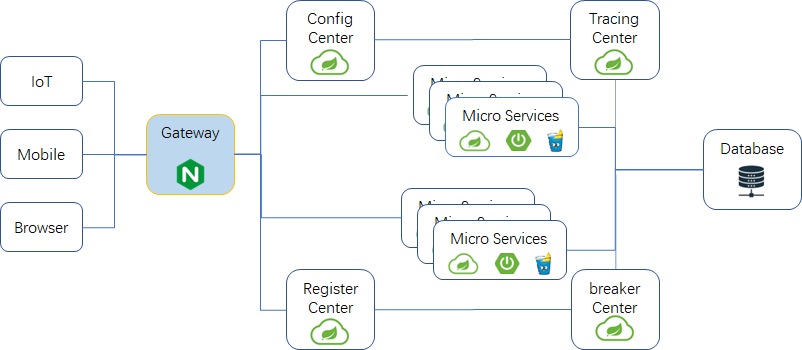
\includegraphics[width=0.9\textwidth]{Img/api 网关.png}
    \caption{微服务网关结构示例}
    \label{fig:api_gateway}
\end{figure}

微服务网关作为微服务后端服务的统一入口,它可以统筹管理后端服务,提供了以下功能:\par

\textbf{路由功能}:路由是微服务网关的核心能力。通过路由功能微服务网关可以将请求转发到目标微服务。在微服务架构中,网关可以结合注册中心的动态服务发现,实现对后端服务的发现,调用方只需要知道网关对外暴露的服务API就可以透明地访问后端微服务。\par
\textbf{负载均衡}:API网关结合负载均衡技术,利用Eureka或者Consul等服务发现工具,通过轮询、指定权重、IP地址哈希等机制实现下游服务的负载均衡。\par
\textbf{统一鉴权}:一般而言,无论对内网还是外网的接口都需要做用户身份认证,而用户认证在一些规模较大的系统中都会采用统一的单点登录(Single Sign On)系统,如果每个微服务都要对接单点登录系统,那么显然比较浪费资源且开发效率低。API网关是统一管理安全性的绝佳场所,可以将认证的部分抽取到网关层,微服务系统无须关注认证的逻辑,只关注自身业务即可。\par
\textbf{协议转换}:API网关的一大作用在于构建异构系统,API网关作为单一入口,通过协议转换整合后台基于REST、AMQP、Dubbo等不同风格和实现技术的微服务,面向Web Mobile、开放平台等特定客户端提供统一服务。\par
\textbf{限流熔断}:在某些场景下需要控制客户端的访问次数和访问频率,一些高并发系统有时还会有限流的需求。在网关上可以配置一个阈值,当请求数超过阈值时就直接返回错误而不继续访问后台服务。当出现流量洪峰或者后端服务出现延迟或故障时,网关能够主动进行熔断,保护后端服务,并保持前端用户体验良好。\par
\textbf{黑白名单}:微服务网关可以使用系统黑名单,过滤HTTP请求特征,拦截异常客户端的请求,例如DDoS攻击等侵蚀带宽或资源迫使服务中断等行为,可以在网关层面进行拦截过滤。比较常见的拦截策略是根据IP地址增加黑名单。在存在鉴权管理的路由服务中可以通过设置白名单跳过鉴权管理而直接访问后端服务资源。\par
\textbf{灰度发布}:微服务网关可以根据HTTP请求中的特殊标记和后端服务列表元数据标识进行流量控制,实现在用户无感知的情况下完成灰度发布。\par

\subsubsection{容器化与服务编排}

\begin{figure}[H]
    \centering
    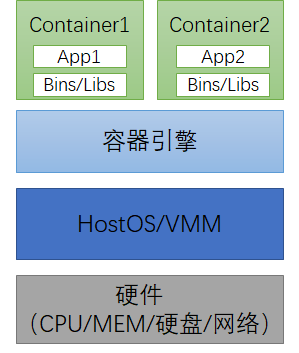
\includegraphics[width=0.6\textwidth, height=0.4\textheight]{Img/container.png}
    \caption{容器化技术}
    \label{fig:container}
\end{figure}

容器化是指将软件代码和所需的所有组件(例如库、框架和其他依赖项)打包在一起,让它们隔离在自己的"容器"中。\par

这样,容器内的软件或应用就可以在任何环境和任何基础架构上一致地移动和运行,不受该环境或基础架构的操作系统影响。容器就像是一个气泡(或者是应用周围的计算环境),把应用和周围环境隔离开来。它相当于是一个功能全面、便于移植的计算环境。\par

容器是取代在平台或操作系统上直接编写代码的一种替代方案,因为在这种旧的方式中,代码可能无法与新环境兼容,使得应用难以移动。如此就可能会产生漏洞、错误和故障,从而需要消耗更多时间进行修复,导致生产力降低和团队产生强烈的挫败感。\par

将应用打包装入可在平台和基础架构之间移动的容器后,只用把该容器移动到某个位置,应用就能在那里成功运行使用,因为容器中包含了成功运行应用所需的一切。\par

服务编排是一种通过简单的拖拉拽式流程编排以及参数配置的方式来进行服务开发的能力,并支持对已开发的服务重新进行组合编排。用户能够在服务编排编辑器内以图形化编排的形式快速地进行服务的开发并扩展出更丰富的业务功能,同时能够与API接口进行绑定,以API的形式对外提供服务。

\subsubsection{服务网格}

服务网格是一个基础设施层,用于处理服务间通信。云原生应用有着复杂的服务拓扑,服务网格保证请求在这些拓扑中可靠地穿梭。在实际应用当中,服务网格通常是由一系列轻量级的网络代理组成的,它们与应用程序部署在一起,但对应用程序透明。\par


\begin{figure}[H]
    \centering
    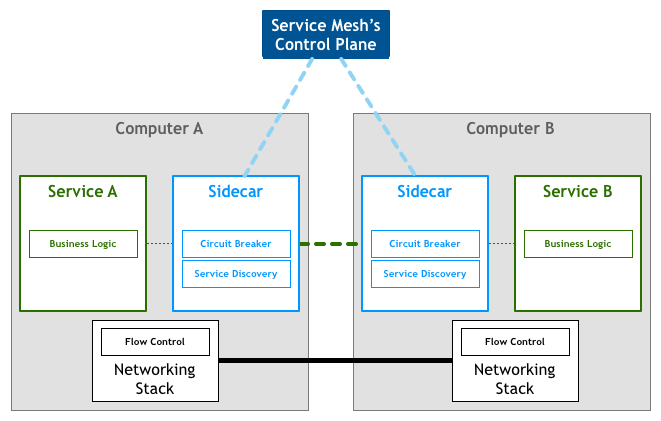
\includegraphics[width=0.9\textwidth]{Img/service mesh.png}
    \caption{服务网格结构示例}
    \label{fig:service_mesh}
\end{figure}

\textbf{非侵入式代理}:服务网格引入的sidecar作为业务微服务的代理,承担了非业务功能:如流量管理、安全认证、监控运维等。sidecar卸载掉了业务微服务的通用功能,使得业务开发人员专注于业务逻辑开发,无需关注其他非业务需求。\par
\textbf{非业务公共能力解耦}:业务微服务功能与sidecar非业务功能分离解耦,业务微服务专注于业务逻辑,与业务逻辑无关的DFX特性,如流量管理、安全认证、监控运维等,全部旁路到sidecar容器统一处理;\par
\textbf{管理面数据面分离}:这也是服务网格的一大优势,通过将控制面与数据面分离解耦,达到不同问题域的解耦目标。控制面只聚焦安全、监控、流量等策略的处理和下发,数据面只聚焦如何执行策略,各自的故障不会相互影响,例如控制面的故障不会影响数据面的流量转发。后面会进一步介绍控制面数据面分离的架构。\par


\subsection{选题意义}

但是微服务集群中的调度问题仍然是影响微服务响应时延的根源问题之一,无论是微服务网关还是服务网格中的sidecar,对于服务调度都是以简单朴素的轮询调度为默认调度方式,不考虑服务实例的现实状态与服务节点的资源状态,同时不考虑服务实例版本不同导致的接口不兼容性等问题。对于服务的调用比较僵硬,对于服务响应效率的提升帮助甚微,同时也不满足当前微服务复杂多变的相互调用需求。

为了解决微服务集群调度问题,实现更好的服务负载均衡达到降低微服务响应时延的目的,本文将研究一种基于当前服务网格及API网关技术,设计实现一个提供更优服务负载均衡策略的的智能网关,从而实现更低的微服务响应时延与更好的服务负载分发,帮助使用者解决微服务集群调度问题,将注意聚焦于服务开发中。
\newpage

\section{国内外本学科领域的发展现状与趋势}

本节将从服务负载计算、服务调度、网关设计三个方面来介绍与本课题相关的研究现状。

\subsection{服务负载计算}

服务负载计算是指通过监控系统对服务集群数据做采集以及对服务节点状态做采集,通过采集到的数据进行定量的计算,得到服务实例当前负载的一个数值。服务负载计算在整个服务调度的过程中占据重要地位,一个好的调度方案离不开合理精准的服务负载计算。现在有不少研究目标在完成更好的服务负载计算与服务调度。\par
Liu~\citep{9112373} 对于负载的计算,提出将负载进行线性归一方法降维处理,通过负载之间的对比来确定最后的负载赋值,同时根据当前服务集群选择的负载均衡策略不同进行不同的服务负载指标获取来获得当前策略下的服务负载值。这种服务负载的计算方式总体上实现简单,在服务集群内部状况简单时可以获得较好的服务负载计算结果,服务调度变得简单。
但是对于服务负载的计算仅考虑一种指标,虽然给出的理由是考虑不同的负载均衡策略,为其提供调度依据,单指标的计算对于服务的总体负载状态描述不够。当关注于服务的内存资源时,如果网络资源较差,但是此时唯一的评判计算标准为内存,那么网络资源差的实例会获得一个低负载状态的声明,在服务调度时就会错误的将请求调度到这个实例中,导致请求响应时延增大,降低了整体的服务响应效率。\par
Amit~\citep{9045136}提出在服务负载计算之前需要对任务进行分类,文章将任务分为数据密集型任务、实时任务和其他任务,针对不同类型的任务给出不同的负载计算依据。比如针对于数据密集型任务,那么磁盘IO速度是负载计算的依据,根据磁盘状态来确定当前实例负载值,然后根据负载值赋予实例不同的权重值去做服务调度。但是这种计算方式没有全面的考虑节点的状态,比如节点的网络状态,会影响数据密集型任务的传输效率。
在这种情况下,分类的效果被削弱,也就是服务负载计算时并没有考虑到所有会影响到服务响应效率的因素,导致服务请求实际提升变小。\par
Cui~\citep{9359175}对于服务负载计算问题采用模型训练的方法解决。通过针对性数据的模型训练,模型可以根据传入的负载数据分析当前服务集群的状态并赋予服务实例合适的负载值供下一步的服务调度使用,通过模型训练的方式可以获得服务集群负载计算的通用方式。但是最终模型的效果取决于服务负载数据集的质量,数据集数据量较小且数据为针对某个服务集群时,得出的模型并不具有普适性,只能服务于特定架构的服务集群。
在这种情况下,模型训练的实际可用范围变小,需要使用者二次训练,违背了设计初衷。\par

\subsection{服务调度}

服务调度是指微服务控制网关对于外部服务请求做出的服务实例选择,微服务控制网关对于服务调度会有默认的调度选择,一般为轮询、随机、最小链接等策略。但是控制网关默认的调度策略并不能很好地适应架构日益复杂的微服务集群。目前不少研究目的为面对外部服务请求时如何进行更好更合适的服务调度,达到更短的服务响应时间。 \par
Nguyen~\citep{s22082869}对于服务调度的方式为将请求事件集中在本地节点,也就是服务请求接受节点进行处理,可以有效地减小通信带来的时间开销。当本地节点的负载值达到预设的阈值时,控制网关会将事件分发给通信时延低的边缘节点进行任务处理。这种处理方式下可以大幅提高响应效率,但是当遇到服务请求峰值时,由于节点负载增长不是瞬时所以在后续任务分配时会将过多的任务分配给当前节点处理,容易导致单个节点负载满值的情况出现。
由于该研究中本地节点同时为服务请求调度节点,所以当本地节点满负载运行时,新的服务请求得不到处理会被直接抛弃,会导致服务响应效率大幅度降低,影响整个系统的负载平衡。 \par
MV4MS~\citep{9284506}对于服务调度的处理方式为先解决服务之间的依赖关系,此研究通过在服务配置文件中显示声明该服务依赖于哪些服务的方式,使得服务之间的调用减少了一次获取服务信息的过程。但是目前微服务集群有着大量相同服务的不同版本服务实例存在,这些服务实例之间存在着一定的服务响应差异,这就导致了服务请求的服务调度时需要考虑服务版本信息。
那么在获取了服务基础信息之后我们还需要获取服务的不同版本对应的信息,使得此研究的服务依赖声明带来的类似服务预处理效果大打折扣。\par
Balancing Load~\citep{10077895}对于服务调度提出了两点优化措施,第一点是提出对服务实例进行版本分流,第二点是实现服务的动态负载均衡策略选择。首先第一点微服务的版本分流,此研究根绝服务实例的负载值计算出服务所在节点的负载值,然后根据负载值给定一个服务权重参考值,在得到服务权重参考值之后根据该参考值计算出同个服务的不同版本的流量修正值。服务控制平面会根据得到的流量修正值修改发向每个服务实例的流量数量,达到平衡负载的作用。
第二点服务的动态负载均衡策略选择,根据第一点中得到的每个服务实例的负载值,对负载值进行均值和方差的计算,根据得到的方差值所在的区间,确定适合该服务版本实例群的负载均衡策略。其中存在的问题是首先第一点对于版本实例分流,默认为不同的服务版本之间服务接口是全部兼容的,但是实际中版本升级会带来一些非兼容性的变化,如果不考虑这些变化,会导致服务请求导向错误的服务实例,最终导致请求出错。对于第二点中提到动态负载均衡策略选择,将方差大于2的所有情况全部赋予同一种
负载均衡策略过于笼统,可以通过自定义负载均衡策略的方式来实现更好的动态选择。

\subsection{网关设计}

\subsubsection{API 网关设计}

\begin{figure}[H]
    \centering
    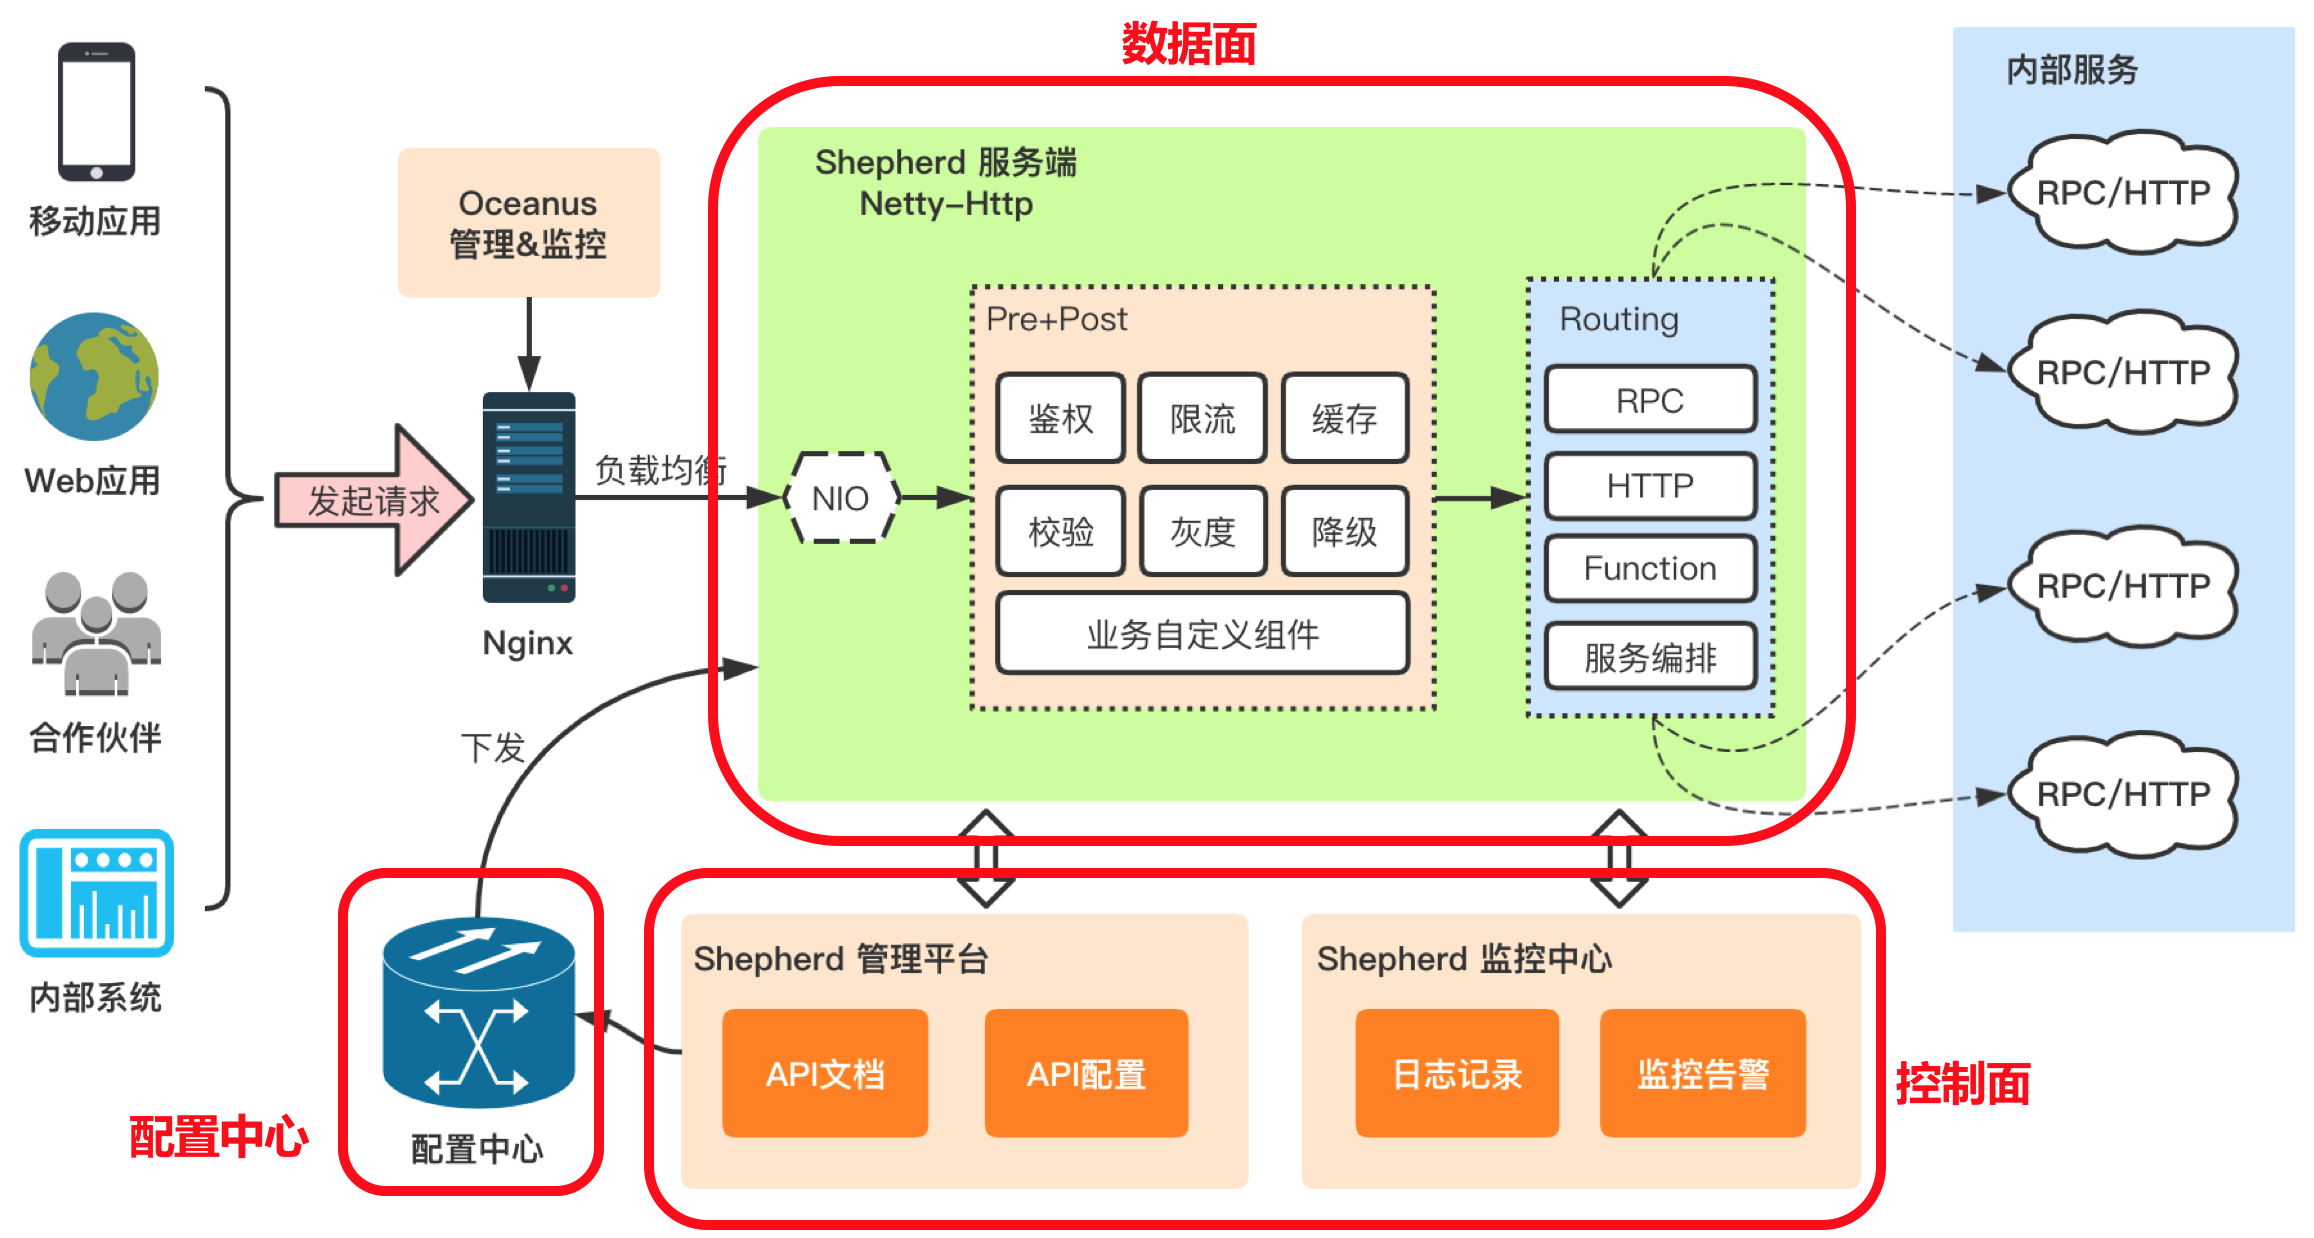
\includegraphics[width=0.9\textwidth]{Img/shepherd.png}
    \caption{shepherd API 网关设计}
    \label{fig:shepherd}
\end{figure}

Shepherd API网关的控制面由Shepherd管理平台和Shepherd监控中心组成。管理平台主要完成API的全生命周期管理以及配置下发的工作,监控中心完成API请求监控数据的收集和业务告警功能。\par

Shepherd API网关的配置中心主要完成控制面与数据面的信息交互,通过美团统一配置服务Lion来实现。\par

Shepherd API网关的数据面也就是Shepherd 服务端。一次完整的API请求,可能是从移动应用、Web应用,合作伙伴或内部系统发起,经过Nginx负载均衡系统后,到达服务端。服务端集成了一系列的基础功能组件和业务自定义组件,通过泛化调用请求后端RPC服务、HTTP服务、函数服务或服务编排服务,最后返回响应结果。\par

\subsubsection{服务网格网关设计}

\begin{figure}[H]
    \centering
    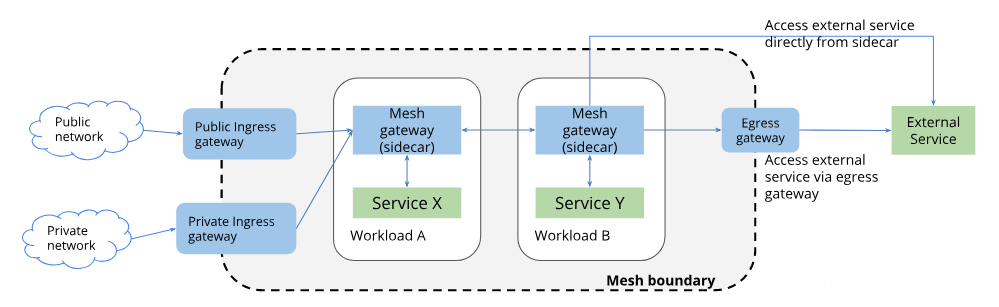
\includegraphics[width=0.9\textwidth]{Img/istio_gateway.png}
    \caption{服务网格网关设计}
    \label{fig:istio_gateway}
\end{figure}

Kubernetes Ingress集群边缘负载均衡, 提供集群内部服务的访问入口,仅支持L7负载均衡, 功能单一
Istio 1.0以前,利用Kubernetes Ingress实现网格内服务暴露。但是Ingress无法实现很多功能:
\begin{itemize}
    \item[(1)] L4-L6负载均衡。
    \item[(2)] 对外mTLS。
    \item[(3)] SNI的支持。
    \item[(4)] 其他istio中已经实现的内部网络功能: Fault Injection,Traffic Shifting, Circuit Breaking, Mirroring。
\end{itemize}
为了解决这些这些问题, Istio在1.0版本设计了新的v1alpha3API。
\begin{itemize}
    \item[(1)] Gateway允许管理员指定L4-L6的设置:端口及TLS设置。
    \item[(2)] 对于ingress 的L7设置, Istio允许将VirtualService与Gateway绑定起来。
    \item[(3)] 分离的好处:用户可以像使用传统的负载均衡设备一样管理进入网格内部的流量,绑定虚拟IP到虚拟服务器上 。便于传统技术用户无缝迁移到微服务.
\end{itemize}

\newpage

\section{课题主要研究内容、预期目标}

\subsection{研究内容}

研究内容主要分成三个部分:1) 基于多维度指标综合的动态负载计算,从多个维度去对服务实例负载进行计算和分析服务实例真正状态。2) 考虑细粒度版本兼容性的路由策略,通过更加细粒度的路由策略,将服务流量分流到更加合适的实例中。 3) 两阶段的服务请求路由机制,通过两种不同着重点的网关之间的相互配合来实现更加灵活的服务请求路由方式。实现这三部分内容并将其融合到一个整体智能网关中,实现一个通用网关。\par

\subsubsection{多维度指标综合的动态负载计算}

对于一个目标为实现智能服务调度的网关,服务负载的计算影响了服务调度时的决策。基于目前研究中对于负载计算选取单维度的方式,我们需要至少在两个方面进行负载计算。首先对服务实例进行服务监控,得到单个实例的负载值以及服务的响应数据,其次对服务节点进行资源监控,获取节点资源及节点响应数据。通过比对两个维度的数据来判断当前实例负载真实状况,赋予该实例准确的负载参考值,为后续权重赋予提供准确的依据。\par
针对负载原始数据的不同,提出一种优先级负载计算方式,根据服务请求的类别来确定负载原始数据的优先级,实现灵活的负载计算。同时负载数据需要考虑时效性,在服务请求的过程中会进行实时的负载计算,且对旧数据进行折损处理,获得准确的实时负载值,提高后续服务调度的准确性。

\subsubsection{细粒度版本兼容下的路由策略}

微服务升级的过程中,考虑到服务稳定性的需求,会出现多个版本的服务并存的现象,版本之间会存在一些非兼容的变化。那么细粒度版本兼容性的路由策略则是为了解决版本之间存在的非兼容性变化提出的,对于多服务共存的调度,分析粒度由服务粒度细化到服务接口粒度。我们将研究对象进行细分之后,按照约定的规则对研究对象进行定义。我们采用语义化版本2.0的规范定义服务版本,RESTful API规范定服务对外接口,
OAS规范定义服务API文档。\par
我们通过细化服务分析粒度的方式实现更加智能的服务调度,将相同服务的不同接口请求分配到与当前服务版本兼容的其余服务中,由于接口兼容性版本区间的不同,服务请求导向不同的服务实例,获得服务负载的平衡。

\subsubsection{两阶段的服务请求路由机制}

\begin{figure}[H]
    \centering
    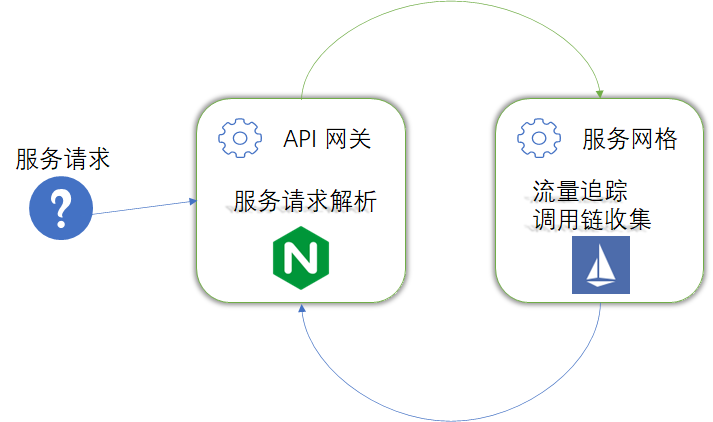
\includegraphics[width=0.9\textwidth]{Img/网关结合.png}
    \caption{网关结合应用}
    \label{fig:gateway_to}
\end{figure}

相对于服务网格中的控制网关,API网关具有更灵活的服务请求解析能力;相较于API网关,服务网格中的控制网关具有更好的流量监控与调用追踪能力。实现灵活的服务负载均衡需要两种网关集合各自的优势来处理服务请求,使用API网关解析服务请求,获取服务版本信息,根据获取的信息计算请求的兼容服务版本区间,将得到的服务实例选择约束传递给服务网格的控制网关;服务网格的控制网关根据服务选择约束信息选择服务实例,并记录服务实例运行状态以及服务内部调用情况。

\subsection{预期目标}

预期目标主要分为三个方面:

\begin{itemize}
    \item[(1)] 设计基于多维度指标的负载计算方法,设计一个服务负载数据归一化方法,将异构的服务集群通过归一化进行统一计算,得到反映服务真实状态的服务负载值。
    \item[(2)] 设计实现一个REST API分析模块,通过对服务API文档的分析获得REST API的兼容版本区间,在服务请求时通过解析请求的REST API信息与(1)中计算得到的服务负载结合分析获得服务调度策略。
    \item[(3)] 实现一个能够结合(1)和(2)的智能网关,主要实现API文档解析,API版本兼容区间分析,服务负载计算,服务调度策略生成,服务调度链生成这几项功能,达到请求最小响应时间与服务集群负载均衡的目标。
\end{itemize}

\newpage

\section{拟采用的研究方法、技术路线、实验方案及其可行性分析}

\subsection{研究方法与技术路线}

\subsubsection{基于多维度指标综合的动态负载计算设计}

多维度指标综合的动态负载计算首先需要做到负载数据收集的全面性。首先要收集服务节点的负载资源数据以及服务节点的总体资源数据,根据目前负载所占总体资源的百分比来确定节点真实负载状态;其次收集服务实例的负载数据,通过多个方面的服务负载数据与多个相同服务的负载数据作比较来确定当前服务状态;还需要结合分析服务节点的负载数据与该节点运行的服务实例负载数据两者之间的关系,确定服务实例的真实状态。 \par
其次要做到对负载数据进行归一化。微服务集群存在服务异构性,不同的服务框架带来的资源消耗存在差异,在进行服务负载计算时需要考虑到这些异构性。需要对不同的服务框架指定不同的服务负载数据项,在这个基础上得到相对客观的服务负载,为后续服务调度提供依据。

\subsubsection{针对细粒度版本兼容性的路由策略设计}

基于研究发现服务集群的路由策略都集中在服务实例的粒度中且没有针对不同版本做服务接口的兼容性分析,当服务出现非兼容性的升级之后,这种调度方式会出现服务请求被调度策略导向错误服务实例版本的情况,服务响应最终出错。\par
首先要解析API文档获取服务的服务接口兼容性信息,将获得的服务接口信息持久化到数据库为后续服务调度工作提供参考信息;其次需要对外部服务请求做信息提取,获得客户端想要访问的API所属的服务实例以及服务版本,通过第一步得到的接口兼容性信息确定可以响应此服务请求的服务实例集合。\par

\subsubsection{基于两阶段的服务请求路由机制设计}

通过API网关统一服务对外接入点,同时通过API网关对外部服务请求做解析,结合前两部分实现的功能完成服务调度的选择。对于API网关首次处理的服务请求,只生成下一跳服务访问的路由,对于服务内部互相调用不给出调度策略,API网关将访问服务的路由送至服务网格控制网关。服务网格控制网关在接收到API网关生成的路由策略后,根据策略将请求转发,同时监控本次请求出现的系统内部服务调用状况并生成服务调用链。\par
服务网格的控制网关将本次服务请求生成的服务调用链进行持久化存储,当相同的服务请求再次到达API网关时,API网关通过查询获得该请求的完整服务调用,在服务请求解析阶段生成完整的服务调用链策略发送至服务网格控制网关。服务网格控制网关在接收到完整服务调度策略之后执行该策略且监控调度过程,当过程出现服务不可达等现象后及时通知API网关同时进行新的服务调用链追踪并更新持久化存储,保持服务调度的正确性。

\subsection{实验方案}

\subsubsection{实验系统}

本课题的实验验证系统分别为istio的bookinfo系统、microservice demo的sockshop系统、复旦实验室的train-ticket系统。

\subsubsection{实验设计}

本课题的实验包括三个部分:\par
\begin{itemize}
    \item[(1)] 对于多维度指标综合的动态负载计算方法,利用模拟请求服务请求部署的服务系统,获取系统的负载数据,通过对数据的分析
    \item[(2)] 对于细粒度版本兼容性的路由策略模块,通过对实验系统的API文档解析获得API接口的版本兼容区间与实际统计版本兼容区间的对比验证正确性,同时检测完整服务调用链中每次调用的版本兼容区间计算正确性。
    \item[(3)] 对于两阶段的服务请求路由机制设计,通过研究方法拟定的过程,检测服务调用链是否能够正确生成以及服务兼容调度链能否正确执行。
\end{itemize}


\subsection{可行性分析}

\textbf{技术可行性:} 本课题进行了较为充分前期文献收集和调研工作,对相关工作的优缺点有了较为充分的认识。在文献调研阶段积累了较为丰富的服务负载计算方式,可以推陈出新,实现更完善的负载计算方式;同时服务版本兼容性计算根据OAS规范与语义化版本规范相结合可以有效的推算出结果;现有的服务网关与服务网格网关可扩展性强,易实现两阶段网关路由请求机制的融合。
\par
\textbf{实验可行性:} 本文所需实验条件由实验室提供,实验系统为经过主流认证的微服务系统,在架构方面能够和业界微服务系统保持一致,具有普适性。
\par
\textbf{环境可行性:} 实验室提供的服务器可以支撑实验运行。\par
综上所述,本课题研究内容完全可行。

\newpage

\section{已有科研基础与所需的科研条件}

\subsection{已有基础}

\begin{itemize}
    \item[(1)] 在之前一年的时间里进行了REST API相关问题的研究,对REST API有一定的了解,具有充足的理论基础,同时对swagger的OAS规范有一定的了解。
    \item[(2)] 对于API网关与服务网格控制网关有专门的学习,积累了网关设计方面的经验。
    \item[(3)] 实验室提供了服务网格所需的服务器等相关开发工具,帮助系统的设计与完成。
    \item[(4)] 实验室配备有完备先进的科研环境,同时有经验丰富的优秀的导师们的指导,和优秀的组内同学的相互协助。
\end{itemize}

\subsection{所需科研条件}

\begin{itemize}
    \item[a)] 在文献研究阶段,使用实验室提供的电子资源检索权限,查阅相关文献;
    \item[b)] 项目实现过程中所需要的服务器资源。
\end{itemize}

\newpage

\section{研究工作计划与进度安排}

\begin{table}[H]
    \centering
    \caption{研究工作计划与进度安排表}
    \begin{tabular}{|c|c|c|}
        \hline
        开始时间 & 结束时间 & 任务安排 \\\hline
        2023年07月 & 2023年08月 & 系统设计技术研究 \\\hline
        2023年09月 & 2023年10月 & 负载计算,兼容分析功能实现 \\\hline
        2023年11月 & 2023年12月 & 网关结合应用与系统实现 \\\hline
        2024年01月 & 2024年02月 & 测试与改善系统 \\\hline
        2024年02月 & 2024年04月 & 总结工作形成论文
        \\\hline
    \end{tabular}
\end{table}

\newpage

\nocite{*}% 使文献列表显示所有参考文献(包括未引用文献)
%---------------------------------------------------------------------------%
% main content
%-
%-> Backmatter: bibliography, glossary, index
%-
\artxifstreq{\artxbib}{bibtex}{% enable bibtex
    \bibliography{Biblio/ref}% bibliography
}{%
    \bibliographystyle{plain}
    \printbibliography% bibliography
}
\end{document}
%---------------------------------------------------------------------------%

